% Naming convention: M_q_maxgen_scale_line-width

\documentclass[crop]{standalone}

\usepackage{tikz,tikzscale}
\usetikzlibrary{calc}

\begin{document}
  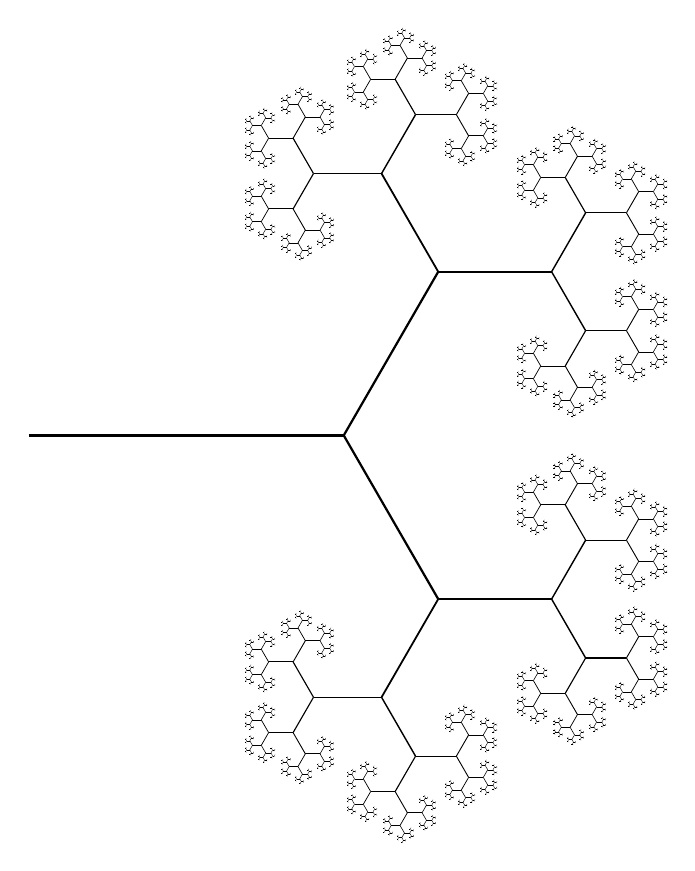
\begin{tikzpicture}[vertex/.style={draw,circle,minimum size=1.3mm,inner sep=0pt,outer sep=0pt,fill=black},scale=4]

    \def\snowflake#1#2#3{
      \newcount\gen
      \pgfmathsetmacro{\M}{#1}
      \pgfmathsetmacro{\q}{#2}
      \pgfmathsetmacro{\lw}{0.8}
      \pgfmathsetmacro{\maxgen}{#3}
      \pgfmathsetmacro{\a}{360/(\M+1)}
      \draw[line width=\lw] (-1, 0) -- (0, 0);
      % \node[vertex] at (-1, 0) {};
      % \node[vertex] at (0, 0) {};
      \def\doit##1##2##3##4{
        \gen=##4
        \ifnum\the\gen<\maxgen {
          \advance\gen by 1
          \pgfmathsetmacro{\prevx}{##1}
          \pgfmathsetmacro{\prevy}{##2}
          \foreach \i in {1,...,\M} {
            \pgfmathsetmacro{\angle}{##3+180+\a*\i}
            \pgfmathsetmacro{\nextx}{\prevx + \q^\gen*cos(\angle)}
            \pgfmathsetmacro{\nexty}{\prevy + \q^\gen*sin(\angle)}
            \draw[line width=\lw^\gen] ({\prevx}, {\prevy}) -- ({\nextx}, {\nexty});
            % \node[vertex,scale=1.5*\lw^\gen] at ({\nextx}, {\nexty}) {};
            \doit{\nextx}{\nexty}{\angle}{\the\gen}
          }
        }
        \fi
      }
      \doit{0}{0}{0}{0}
    }

    \snowflake{2}{0.6}{11}

  \end{tikzpicture}
\end{document}
